\section{Analysis and Design} \label{sec:Design}

Seeing that this is a system dealing with finance, it would make sense to treat
the categories as if they were accounts. And, in order to make sure to imbue
this system with knowledge acquired by more experienced programmers, it makes
sense to make use of patterns.

% maybe move to appendix
It is also useful at this point to make a distinction between the types of
classes used to model the domain between three possible kinds: the first are
the classes which model the interaction between the system and its actors --
these are called \emph{boundary classes}; the second kind are those classes
which model information and/or behaviour or some concept or phenomenon -- these
will be called \emph{entity classes}; and lastly, there are those classes which
model transactions, coordination, control and sequencing of other objects --
which are known as \emph{control classes} (Jacobson et al., 1999,
\cite[cited][pp.~198-201]{bennett2010object}).

The first analysis patterns which seem appropriate are the \emph{Account}
pattern, used to create the \emph{Category} entity class, and the
\emph{Quantity} pattern for the \emph{Amount} entity class
(\cite[][Sections~6.1~\&~3.1]{fowler1997analysis}):
\begin{figure}[ht!]
  \begin{center}
    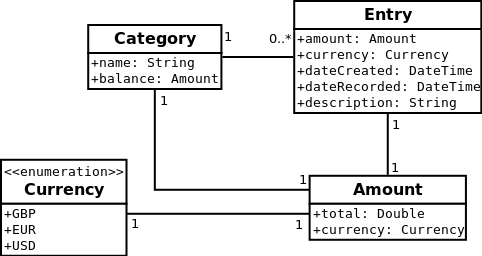
\includegraphics[width=11cm]{./contents/img/Class_Diagram_-_Categories_and_Amount.png}
  \end{center}
  \caption{}
  \label{fig:ClassDiagram.CategoriesAndAmount}
\end{figure}
\FloatBarrier

As implied by the diagram above, the \emph{Category} class will be associated
with instances of the \emph{Entry} class, and will keep track of the balance
made up of the sum of \emph{Amount}'s of each entry. This is done so that the
only way to change the total of a category is by adding positive or negative
entries to it -- for example, to indicate a credit to a category, a negative
entry can be added to it.

Another design choice which can be observed in Figure
\ref{fig:ClassDiagram.CategoriesAndAmount} is that the \emph{Amount} class also
possesses an attribute for currency. This has been designed so as to allow for
the possibility of extending the design to keep track of transactions in
multiple currencies, although it was not a specific requirement. Initially,
there will only be a single default currency which shall be set at runtime.

The next step is to provide a way for these entries to be added to categories.
For this to happen, there needs to be a constraint in to ensure that double
entry happens every time a change needs to be made to a category. One of the
ways to achieve this is to apply the \emph{Transaction} pattern
(\cite[][Section~6.2]{fowler1997analysis}):
\begin{figure}[ht!]
  \begin{center}
    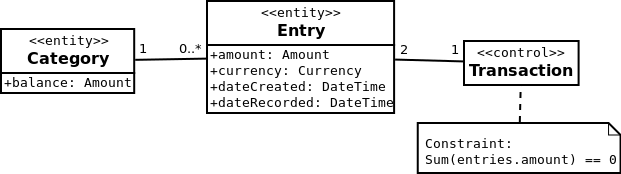
\includegraphics[width=14cm]{./contents/img/Class_Diagram_-_Transaction.png}
  \end{center}
\end{figure}
\FloatBarrier

After having determined the analysis patterns which shall be employed, it makes
sense to dive into a deeper analysis of the use cases described in Chapter
\ref{sec:Requirements}. At this point the objective will be to start modelling
classes based on concepts or things found in the problem domain. This will be
done in the following subsections.

\subsection{Create Manual Entry} \label{sec:AnalysisAndDesign.ManualEntry}

%TODO: check if this diagram still makes sense after implementation
The \emph{Create Manual Entry} use case, which allows a
user to input financial transactions individually using a specific interface,
can be modelled as follows (Figure \ref{fig:CommDiagram.CreateManualEntry}):
\begin{figure}[ht!]
  \begin{center}
    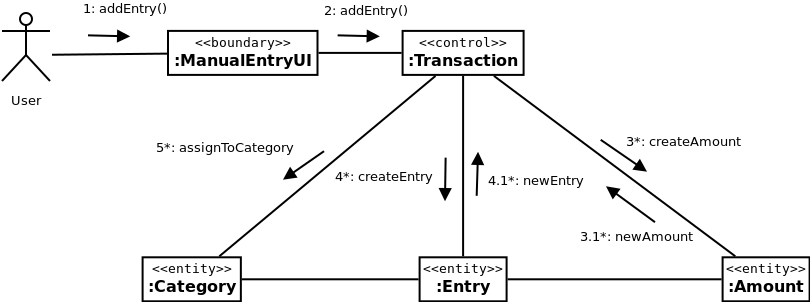
\includegraphics[width=16cm]{./contents/img/Comm_Diagram_-_Manual_Entry.png}
  \end{center}
  \caption{Communication Diagram for the \emph{Create Manual Entry} use case}
  \label{fig:CommDiagram.CreateManualEntry}
\end{figure}
\FloatBarrier

As the diagram above indicates, the \emph{Transaction} class is responsible for
the creation of new instances of \emph{Entry} and \emph{Amount}, which then get
assigned to the \emph{Category} instances involved in the transaction. Although
\emph{Transaction} was originally thought of as \emph{control class}, it was
decided that it would be beneficial to save the transaction information, so it
was made into an \emph{entity class} instead. This process assumes that all
categories already exist, and a separate diagram will be created for the
creation of a new category.


\subsection{Upload Statement} \label{sec:AnalysisAndDesign.UploadStatement}

The user should be able to upload their bank statements, provided that they are
in a suitable format. The specifics of the format will be described in the
implementation phase, together with more information on how to encapsulate as
much as possible the complexities related to formatting of this information.
For the analysis and design phases, the emphasis will be on modelling the
objects and their interactions. The diagram (Figure
\ref{fig:CommDiagram.CreateManualEntry}) below illustrates this process:
\begin{figure}[ht!]
  \begin{center}
    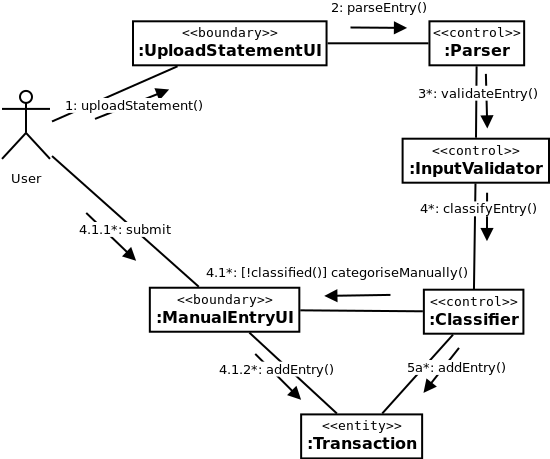
\includegraphics[width=16cm]{./contents/img/Comm_Diagram_-_Upload_Statement.png}
  \end{center}
  \caption{Communication Diagram for the \emph{Upload Statement} use case}
  \label{fig:CommDiagram.CreateManualEntry}
\end{figure}
\FloatBarrier

As can be seen in the diagram above, the process is spread among many classes.
After the user uploads the statement, the loaded raw input will be sent to a
\emph{Parser} which will separate it according to the columns into the
appropriate fields and line items. Then, what is now a collection of statement
line items will be passed on to an \emph{InputValidator} to make sure the user
input is valid at this point. Lastly, the resulting validated entries will be
sent down to a \emph{Classifier}, which will initiate the transaction to
allocate the entries to categories.
